\setcounter{figure}{0}
\renewcommand{\thefigure}{A.\arabic{figure}}
\setcounter{table}{0}
\renewcommand{\thetable}{A.\arabic{table}}


\section{Inferenza Statistica e Feature Selection}
\label{app:stat_inference}

La presente appendice formalizza il framework metodologico adottato per l'analisi esplorativa e la selezione delle variabili. Il protocollo è stato progettato per garantire la robustezza delle stime in presenza di grandi campioni ($N > 30.000$) e per mitigare il rischio di scoperte false positive (Type I errors) derivanti da test di ipotesi multipli.

\subsection{Verifica delle Assunzioni Distributive}

La validità dei test parametrici è subordinata al rispetto delle assunzioni di normalità e omoschedasticità. Data la sensibilità dei test di bontà dell'adattamento (*goodness-of-fit*) alla dimensione campionaria, è stata implementata una strategia adattiva.

\subsection{Test di Normalità Ibrido}
Per la verifica dell'ipotesi nulla di normalità $H_0: F(x) \sim \mathcal{N}(\mu, \sigma^2)$, è stato adottato un criterio decisionale basato sulla numerosità campionaria $N$:

\begin{itemize}
    \item \textbf{Per $N < 5000$ (Shapiro-Wilk):} Si utilizza la statistica $W$ di Shapiro-Wilk, che valuta la correlazione tra i dati ordinati e i punteggi normali attesi. Questo test offre la massima potenza statistica per campioni ridotti o medi.
    \item \textbf{Per $N \ge 5000$ (Jarque-Bera):} Al crescere di $N$, il test di Shapiro-Wilk tende a rifiutare $H_0$ anche per deviazioni trascurabili dalla normalità (paradosso della potenza eccessiva). In questo regime asintotico, si adotta il test di Jarque-Bera, che si basa sui momenti terzi e quarti della distribuzione empirica (skewness $S$ e kurtosis $K$):
    \begin{equation}
        JB = \frac{N}{6} \left( S^2 + \frac{(K-3)^2}{4} \right)
    \end{equation}
    Il test verifica asintoticamente se i momenti campionari coincidono con quelli di una distribuzione normale ($S=0, K=3$).
\end{itemize}

\begin{figure}[H]
    \centering
    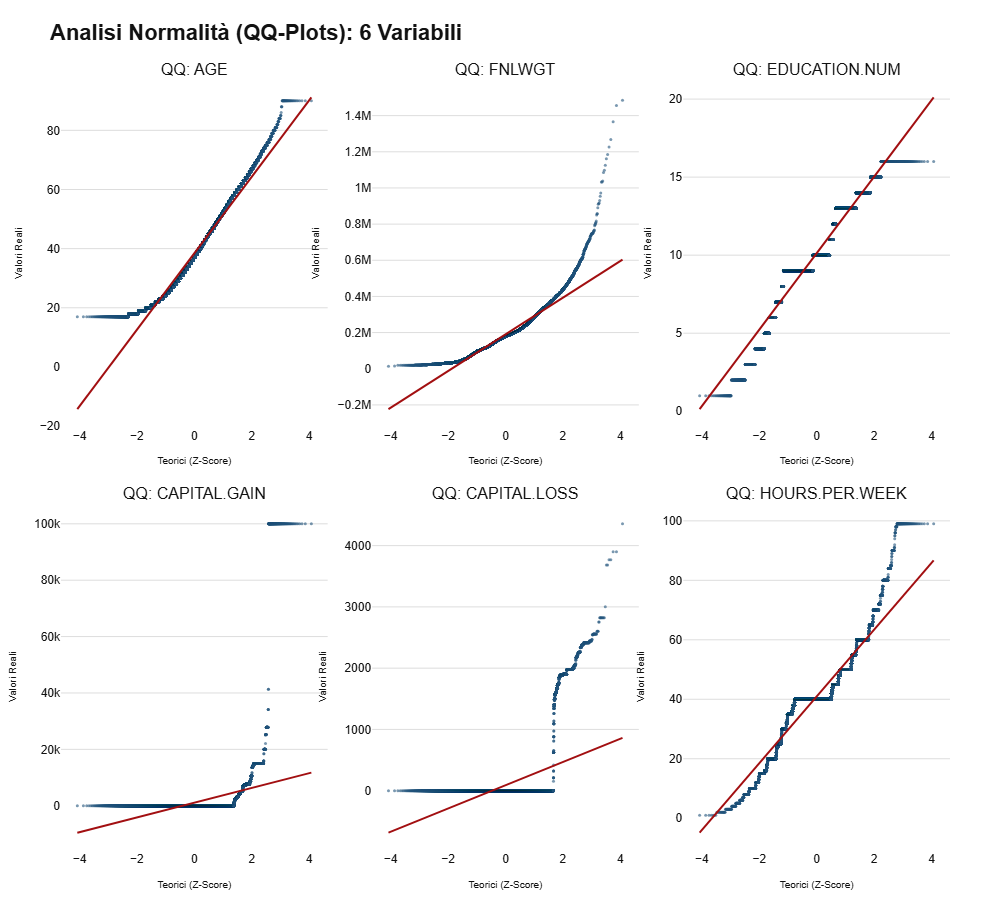
\includegraphics[width=1\linewidth]{figures/qq.png}
    \caption{\textbf{QQ Plot}  Nel complesso, l’analisi evidenzia che la maggior parte delle variabili non segue una distribuzione normale, suggerendo l’eventuale necessità di trasformazioni o l’utilizzo di metodi statistici robusti o non parametrici nelle analisi successive.}
    \label{fig:qq.png}
\end{figure}

\subsection{Omoschedasticità}
L'assunzione di omogeneità delle varianze tra i gruppi è stata verificata mediante il \textbf{test di Levene} centrato sulla mediana (metodo Brown-Forsythe). Tale approccio è preferito al test di Bartlett in quanto significativamente più robusto alle violazioni della normalità distributiva.

\subsection{Test di Ipotesi e Correzione FDR}

La selezione del test statistico per valutare la relazione tra le feature $X_i$ e la variabile target $Y$ avviene dinamicamente secondo l'albero decisionale riportato in Tabella \ref{tab:test}.

\begin{table}[H]
\centering
\begin{tabular}{lccc}
\toprule
\textbf{Tipologia $X_i$} & \textbf{Normalità} & \textbf{Omoschedasticità} & \textbf{Test Statistico} \\
\midrule
Categorica & - & - & $\chi^2$ di Pearson \\
Numerica & Sì & Sì & $t$-test di Student / ANOVA \\
Numerica & Sì & No & $t$-test di Welch / Welch ANOVA \\
Numerica & No & - & Mann-Whitney $U$ / Kruskal-Wallis \\
\bottomrule
\end{tabular}
\caption{Matrice decisionale per la selezione dei test di ipotesi.}
\label{tab:test}
\end{table}

\subsection{Controllo del False Discovery Rate (FDR)}
Conducendo $m$ test simultanei (uno per ogni feature), la probabilità di commettere almeno un errore di I tipo (FWER) aumenta drasticamente. Per ovviare a ciò senza incorrere nell'eccessivo conservatorismo della correzione di Bonferroni, si è applicata la procedura di \textbf{Benjamini-Hochberg}.
\noindent
Dato l'insieme dei $p$-value ordinati $p_{(1)} \le p_{(2)} \le \dots \le p_{(m)}$, la procedura identifica il più grande indice $k$ tale che:
\begin{equation}
    p_{(k)} \le \frac{k}{m} \alpha
\end{equation}
Tutti i test con $p$-value $p_{(i)} \le p_{(k)}$ vengono dichiarati significativi, controllando il tasso atteso di false scoperte al livello $\alpha=0.05$.

\subsection{Stima della Dimensione dell'Effetto (Effect Size)}

La sola significatività statistica ($p < \alpha$) non implica rilevanza pratica, specialmente in presenza di grandi dataset dove differenze infinitesimali risultano statisticamente significative. L'analisi è stata integrata con metriche di \textit{Effect Size} standardizzate.

\subsection{Vargha-Delaney $\hat{A}_{12}$ (Non-Parametrico)}
Per le variabili numeriche che non soddisfano l'assunzione di normalità (e.g., analizzate con Mann-Whitney $U$), è stata calcolata la misura di \textit{Stochastic Superiority} $\hat{A}_{12}$ di Vargha e Delaney. Questa metrica stima la probabilità che un valore estratto casualmente da un gruppo sia maggiore di un valore estratto dall'altro:
\begin{equation}
    \hat{A}_{12} = \frac{R_1/n_1 - (n_1+1)/2}{n_2}
\end{equation}
dove $R_1$ è la somma dei ranghi del primo gruppo. L'interpretazione si basa sulla distanza dall'ipotesi nulla (0.5):
\begin{itemize}
    \item Trascurabile: $| \hat{A}_{12} - 0.5 | < 0.06$
    \item Piccolo: $0.06 \le | \hat{A}_{12} - 0.5 | < 0.14$
    \item Medio: $0.14 \le | \hat{A}_{12} - 0.5 | < 0.21$
    \item Grande: $| \hat{A}_{12} - 0.5 | \ge 0.21$
\end{itemize}

\subsection{Cramer's $V$ (Categorico)}
Per le tabelle di contingenza derivanti dal test $\chi^2$, l'intensità dell'associazione è stata misurata tramite la V di Cramer, normalizzando la statistica $\chi^2$ rispetto alla dimensione campionaria $N$ e ai gradi di libertà minimi ($q = \min(r-1, c-1)$):
\begin{equation}
    V = \sqrt{\frac{\chi^2}{N \cdot q}}
\end{equation}

\subsection{Algoritmo di Feature Selection}

Sulla base delle inferenze prodotte, è stato definito un algoritmo di selezione volto a identificare i predittori ottimali per la modellazione successiva. Una feature viene candidata all'esclusione se soddisfa almeno una delle seguenti condizioni critiche:

\begin{enumerate}
    \item \textbf{Criterio di Sparsità:} Percentuale di valori mancanti $> 60\%$.
    \item \textbf{Criterio di Varianza:} Varianza nulla (feature costante).
    \item \textbf{Criterio di Inferenza (Rumore):} $p\text{-value}_{adj} > 0.05$.
    \item \textbf{Criterio di Rilevanza (Effect Size):} La feature risulta statisticamente significativa ma l'effetto stimato è classificato come "Trascurabile" (e.g., Vargha-Delaney $\hat{A}_{12} \approx 0.5$).
\end{enumerate}

\noindent
L'applicazione di tale protocollo al dataset in esame ha evidenziato la non significatività della variabile \texttt{fnlwgt} ($p_{adj}=0.08$) e la scarsa rilevanza pratica di \texttt{capital.loss} ($\hat{A}_{12}=0.466$, effetto trascurabile), suggerendone l'esclusione per parsimonia del modello.
